\documentclass[]{report}[12 pt]
\usepackage{geometry}
\usepackage{amsmath}
\usepackage{graphicx}
\usepackage{hyperref}
\geometry{margin= 1.5 cm}
\begin{document}
	\begin{titlepage}
	\begin{center}
		\vspace*{1cm}
		
		\Huge
		\textbf{Laboratory Report}
		
		\vspace{0.5cm}
		\LARGE
		X Ray Diffraction\\
		\vspace{0.5cm}
		\textbf{Guide: Prof. Sangita Bose}
		
		\vspace{1.5cm}
		
		\textbf{A R Bathri Narayanan}\\
		Roll no: P0211501\\
		UM DAE Centre for Excellence in Basic Sciences
		
		\vspace{3 cm}
		
		Report presented for the\\
		Advanced Physics Laboratory Course (PL 701)
		
		\vspace{0.8cm}
		
		
\includegraphics[width=0.4\textwidth]{cebs.jpg}
		
		\Large
		School of Physical Sciences\\
		UM-DAE Centre for Excellence in Basic Sciences\\
		Mumbai, MH, India\\
		\today
		
	\end{center}
\end{titlepage}

\section*{Objectives:}
\begin{enumerate}
	\item To study the IR characteristics of plasma with Langmuir probe.
	\item To study the dependence of obtained IR graph by varying pressure, voltage bias and resistance.
\end{enumerate}

\section*{Theory:}

\section*{Observations:}
We shall use a step voltage, so that we can study the IR characteristics in one shot.

\begin{center}
	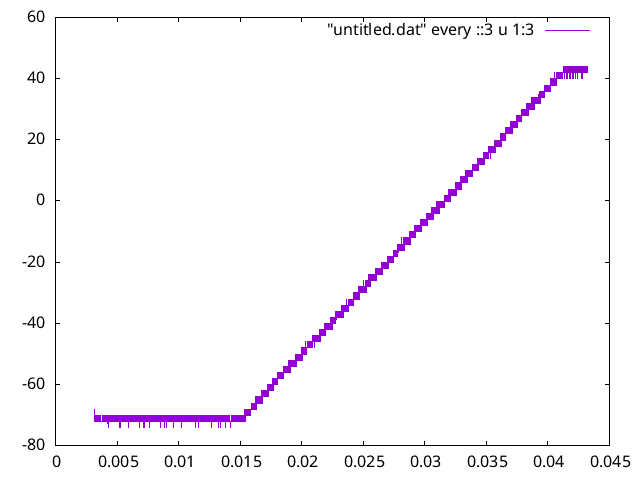
\includegraphics[width=10cm]{voltage}\\
	The step voltage take, the time is on x-axis and the voltage is on Y axis.
\end{center}
\subsection*{Variation of Pressure}
\begin{center}
	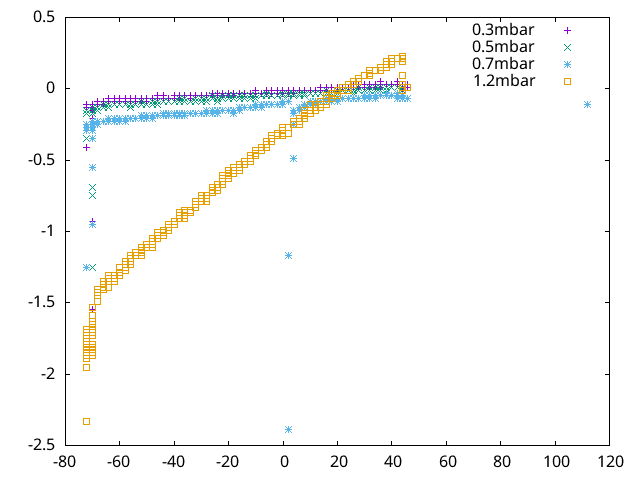
\includegraphics{variationpressure.png}\\
	V-I characteristics of the Plasma as we vary pressure.
\end{center}
We can see a non-linear variation of the graph as we increase the pressure. It first decreases and then increases. The reason might be due to the Paschen effect.
\[V = \frac{Bpd}{ln\bigg(\frac{Apd}{ln(1+\gamma^{-1})}\bigg)}\] 
At constant V, as we vary pressure, at first, it decreases and then it increases logarithmically.
\subsection*{Flipping the circuit}
\begin{center}
	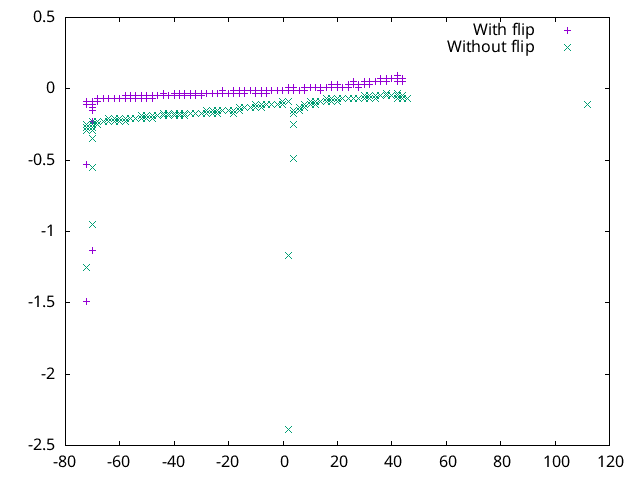
\includegraphics{flipping.png}\\
	V-I characteristics of the plasma as we flip the circuit.
\end{center}

\subsection*{Variation of Bias Voltage}
\begin{center}
	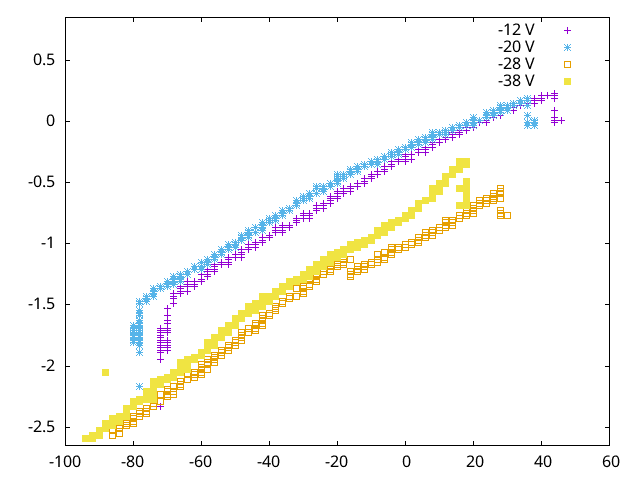
\includegraphics{variationbias.png}\\
	V-I characteristics of the plasma as we vary the bias voltage.
\end{center}

\subsection*{Variation of Resistance}
\begin{center}
	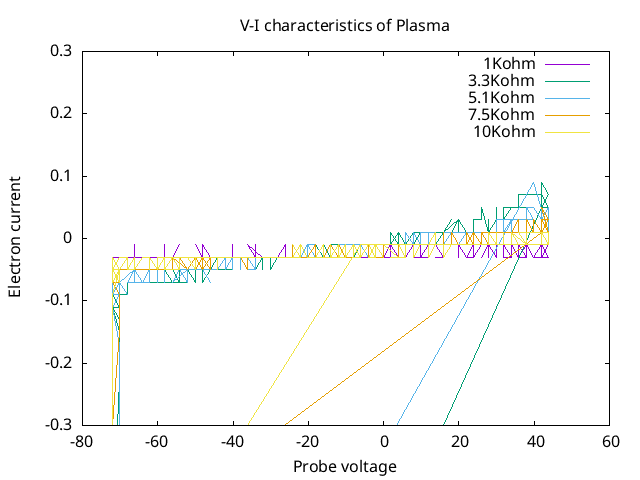
\includegraphics{variationresistance.png}\\
	V-I characteristics of the plasma as we vary resistance.
\end{center}

\section*{Results:}

\end{document}